%%% -*- coding: utf-8 -*-
\newpage

\chapter{Introduction}
\label{chap:introduction}

\section{Motivations}
\label{sec:motivations}
Different games were historically used to benchmark and explore Artificial Intelligence algorithms. In the last twenty years, several games like Chess, Checkers, Go, Backgammon and even Atari games were solved~\cite{Kocsis2006}, with algorithms reaching strategies that could win from professional players. To solve these style of games, a player has to take a decision given a perfect information scenario. In other words, all the information concerning the game state is available to the player: board configuration in case of board games, screen state in case of Atari games. Since there is no hidden information about the game, a brute-force search can retrieve the best action~\cite{Billings1998} with confidence.

But real life is not like that. According to von Neumann, founder of modern game theory, “real life consists of bluffing, of little tactics of deception, of asking yourself what is the other man going to think I mean to do. And that is what games are about in my theory.”~\cite{Bronowski1973}

In poker, a player’s private cards give asymmetric information about the state of the game. Each player sees a different state of the game, and none of them sees the complete state. This is why poker is called an Imperfect Information game and why it's hard to model and solve. Even if a better strategy is played, it can lose from a worse strategy because it has better cards, or it has bluffed or even changed strategy. To give a perspective, an example of an incomplete information board game is Battleship, while Chess is a perfect information game.

Along with that, the number of possible states in Heads-Up No-Limit Texas Hold’em Poker is approximately $10^{160}$ . Heads-Up means there are only two players in the table, so the number of states in a multiplayer table is even bigger. In comparison, chess and backgammon have $10^{47}$ and $10^{20}$ game states respectively~\cite{Johanson2013}. The universe has approximately $10^{80}$ atoms.

Limit Texas Hold’em Poker, a game variation in which players can only raise bets to a fixed amount, have around $10^{13}$ decision points in a heads-up game, and for that, it is a lot easier to solve a Limit poker variant. In fact, it was solved in 2015 by the Cepheus algorithm, developed by the Computer Poker Research Group at University of Alberta, and a joint effort with Oskari Tammelin, a Finnish software developer~\cite{Tammelin2015}.

Furthermore, card games have an element of chance when the deck is shuffled, before dealing the cards. Also, in Texas Hold'em early rounds (named pre-flop, flop, and turn) players have to act before seeing all dealt cards. A player's chance might change when a public card is revealed. This is why poker is classified as a stochastic game, in other words, not deterministic. An example of a stochastic board game is Backgammon, while Chess and Checkers are examples of deterministic games.

Real-world problems, like network and airport security, financial and energy trading, traffic control, routing, business negotiations and forecasting (weather, politics, etc) involve decision making with imperfect information and high-dimensional information states with a huge number of decision points ~\cite{Silver2016}, like poker. Those problems have some characteristics that require intelligent behavior~\cite{Billings1998}. We can map many of those characteristics to poker aspects:

\vspace{0.5cm}
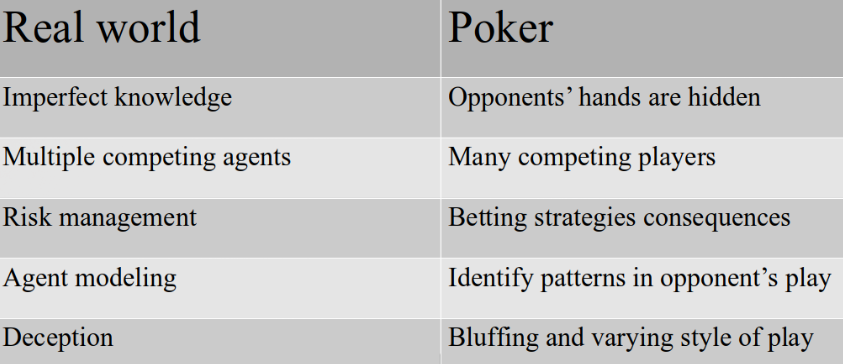
\includegraphics[scale=0.4]{real-world}
\vspace{0.5cm}

An optimal solution to these problems would be a Nash equilibrium, a strategy that if an agent deviates, it loses. If it follows, it wins. If an opponent also follows, both tie. Simple machine learning methods achieve near-optimal solutions to perfect information games but fail to converge in imperfect information games. Using a controlled environment such as poker, allows one to measure progress in a domain where simple machine learning does not converge to near-optimal solutions.

\section{Goals}
\label{sec:goals}

The imperfect information property, the stochastic property, along with the size of the game makes solving of multiplayer No-Limit Texas Hold’em Poker an interesting milestone for Computer Science, not reached until now. This work proposes Pucker, a framework to help scientists reach this goal, providing a consistent simulation of the game, storage of past scenarios in an efficient way, a learning  and prediction strategy for machine learning algorithms, and some examples of algorithms to help the development of better strategies.

The best Pucker agent is inspired by reinforcement learning, similar to David Silver's work ~\cite{Silver2016}, but adds domain knowledge and state abstraction to learn multiplayer No Limit Texas Hold'em. In the end, we show how to measure progress and display a consistent evaluation of the agent's incremental learning.

Unfortunately, there are several caveats in learning from a generated dataset. A learning model requires a fine representation of poker state, with information such as private and public cards, previous opponents' actions, and any known public information the enables a gradient descent model to approach incremental learning. Also, the training data obtained from simulation of deterministic weak players are not sophisticated enough to generate a model competitive against serious players.

To deal with these challenges, we propose a high dimensional representation composed with most of the information used by professional players, along with statistical features built by simulation of future rounds, that improved early stage poker actions such as flop actions. Also, we improved the dataset by running multiple phases of learning, whereas the first phase relies on data generated by deterministic players, and further phases learn from data generated from deep learning sophisticated players. Finally, we propose a method inspired by genetic algorithms, to prevent reaching a local best response by generating populations of algorithms from the most winners. In the end, we acknowledge that the last descendants of this population are capable of better actions.

In summary,  our contributions are:

\begin{itemize}
  \item A framework to build Texas Hold'em agents;
  \item A simulation of the game that can be used to generate input dataset in an efficient way;
  \item Several deterministic players used to generate initial data and measure learning progress;
  \item A state representation that players can use to learn best actions;
  \item A learning and prediction neural network that leverages reinforcement learning to learn a multi-step game such as poker;
\end{itemize}


\section{Dissertation Structure}
\label{sec:organization}

The remainder of this thesis is organized as follows:

\begin{itemize}
  \item Chapter~\ref{chap:background} we describe \textbf{how to play poker} and the \textbf{related work};
  \item Chapter~\ref{chap:learning} shows how \textbf{neural networks} work to gradually improve its predictions and how we used reinforcement learning to adapt the model to multi-step games;
  \item Chapter~\ref{chap:architecture} describes the project \textbf{architecture}, simulation, data storage, learn and predict modules;
  \item Chapter~\ref{chap:evaluation} presents the experiments and the associated \textbf{results};
  \item Chapter~\ref{chap:conclusions} presents some \textbf{concluding remarks} and directions for the future work;
\end{itemize}

%%% Local Variables:
%%% mode: latex
%%% TeX-master: thesis.tex
%%% End:
